\documentclass[10pt]{article}
\usepackage{icmlko}

\icmlmeta{IP 파운데이션 월드모델}{152}{읽히는 축은 안 맞고 맞는 축은 안 읽힌다}{노트 151이 과제 78을 임계 경로에 올렸다. 자동 태거를 열어 보니 열 축이 대각선으로 완전히 갈려 있었다 --- 겹치는 것이 하나도 없다}

\begin{document}

\twocolumn[
\icmlheader

\begin{abstract}
노트 151이 팝업 유보 59건의 벽을 갈랐다 --- 막는 것은 집계 필터가 아니라
\textbf{사람이 축을 매긴 건수}였다. 그러면 자동 태거가 임계 경로다. 열어
봤다. 태거는 열 축을 매기고 교차검증 $\rho$ 가 축마다 적혀 있다. 정렬해
보니 \textbf{제일 잘 읽는 셋이 체험 밀도(0.587) · 포토존(0.513) · 계절
적합(0.512)이고, 제일 못 읽는 다섯이 굿즈 규모(0.414) · 미디어
푸시(0.249) · 장소 노출(0.187) · 입장 마찰(0.181) · 타깃 폭(0.151)이다.}
뒤의 다섯이 정확히 \textbf{공유 축 다섯} --- 전 도메인이 쓰는 그 다섯이다.
그래서 반대쪽을 쟀다. 사람이 매긴 팝업 67건에서 축과 라벨의 상관을 보니
\textbf{장소 노출 $+$0.441 · 타깃 폭 $+$0.401 · 미디어 푸시 $+$0.304 ·
굿즈 규모 $+$0.280 · 입장 마찰 $-$0.271}로 상위 다섯이 또 정확히 공유
다섯이다. 팝업 전용 다섯은 $+$0.209 아래다. \textbf{두 순위가 겹치는 축이
하나도 없다} --- $|$라벨 상관$|$ 과 태거 $\rho$ 의 순위 상관이
\textbf{$-$0.685}이고, 무리 평균으로는 공유 다섯이 라벨 0.339 · 태거 0.236,
팝업 전용이 라벨 0.140 · 태거 0.455다. \textbf{이것이 노트 133의 붕괴를
기제까지 설명한다} --- 자동 태깅으로 팝업이 $+$0.4562에서 $+$0.1150으로
무너진 것은 태거가 나빠서가 아니라 \emph{하필 신호가 있는 다섯 칸에만}
채워 넣기 때문이다. 다만 과대 해석은 막아 둔다. 무리 \emph{안에서는} 이
관계가 안 보인다(공유 안 $-$0.20, 전용 안 $+$0.10) --- $-$0.685는 거의
전부 무리 사이 효과이고, 그 무리 나누기는 예전에 부분적으로 예측력을 보고
정한 것이다. 그러므로 ``쓸모 있어서 못 읽힌다''는 법칙은 세우지 않는다.
세우는 것은 운영 사실 하나다 --- \textbf{우리가 실제로 쓰는 다섯이 태거가
제일 못하는 다섯이고, 그래서 지금 태거로는 팝업 표본을 못 늘린다.}
\end{abstract}
]

\begin{figure*}[t]
\centering
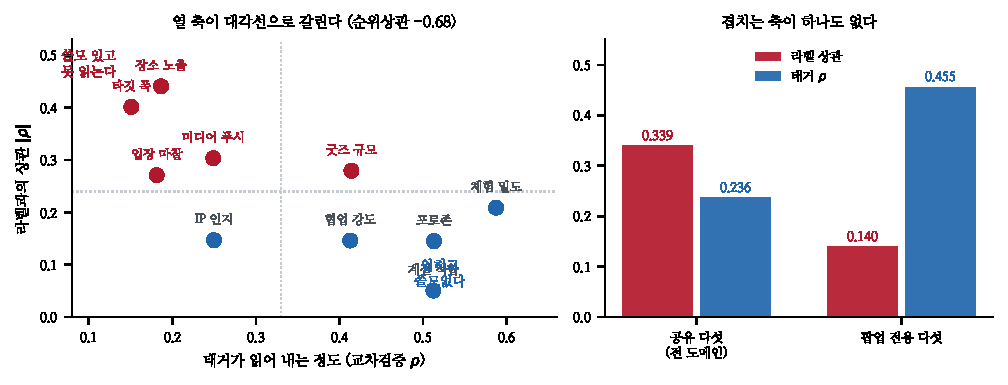
\includegraphics[width=\textwidth]{figs/read.pdf}
\caption{왼쪽 --- 열 축이 대각선으로 갈린다. 오른쪽 --- 두 무리에 겹치는
축이 하나도 없다.}
\end{figure*}

\section{태거가 못 읽는 다섯}

\begin{table}[t]
\centering\tsize
\caption{자동 태거 교차검증(학습 95건). 라벨 상관은 사람이 매긴 67건.}
\begin{tabular}{lrrl}
\toprule
& 태거 $\rho$ & 라벨 $|\rho|$ & \\
\midrule
체험 밀도 & \textbf{.587} & .209 & 팝업 전용 \\
포토존 & \textbf{.513} & .145 & 팝업 전용 \\
계절 적합 & \textbf{.512} & .051 & 팝업 전용 \\
협업 강도 & .413 & .146 & 팝업 전용 \\
IP 인지 & .250 & .147 & 팝업 전용 \\
\midrule
굿즈 규모 & .414 & .280 & \textbf{공유} \\
미디어 푸시 & .249 & .304 & \textbf{공유} \\
장소 노출 & .187 & \textbf{.441} & \textbf{공유} \\
입장 마찰 & .181 & .271 & \textbf{공유} \\
타깃 폭 & .151 & \textbf{.401} & \textbf{공유} \\
\bottomrule
\end{tabular}
\end{table}

\claimx{\textbf{두 순위가 하나도 안 겹친다.} 라벨 상관 상위 다섯이 공유
다섯이고, 태거 $\rho$ 상위 다섯이 팝업 전용 다섯이다. 우연히 이렇게
갈릴 확률은 $1/\binom{10}{5}=1/252$다.}{공유 다섯은 ``전 도메인에 매길
수 있는 것''으로 고른 것이라 추상적이고, 팝업 전용 다섯은 기획서에 대개
숫자로 적혀 있다(``포토존 3개'', ``여름 한정''). 그 차이가 원인일 수 있다.}

\claimx{\textbf{퍼짐 탓이 아니다.} 태거가 못 맞히는 이유가 ``맞힐 변이가
없어서''일 수 있는데, 두 무리의 라벨 표준편차가 1.102 대 1.064로 거의
같다.}{교차검증 $\rho$ 는 태거의 성능이고, 사람 라벨 자체의 잡음도 섞여
있다. 다만 라벨이 더 잡음이라면 라벨 상관도 같이 깎여야 하는데 오히려 높다.}

\section{노트 133의 붕괴가 설명된다}

\begin{table}[t]
\centering\tsize
\caption{팝업 $\rho$(노트 133).}
\begin{tabular}{lrl}
\toprule
사람이 매긴 축 & $+$.4562 & \\
\textbf{자동 태깅으로 채움} & \textbf{$+$.1150} & \textbf{$-$0.341} \\
\bottomrule
\end{tabular}
\end{table}

\claimx{\textbf{태거가 나빠서가 아니라 하필 그 다섯이라서다.} 채워 넣는
칸이 공유 다섯이고 그 다섯의 태거 $\rho$ 평균이 0.236이다. 즉 신호가 제일
센 칸에 제일 흐린 값을 넣는다.}{태거의 전체 평균 $\rho$ 는 0.346으로
나쁘지 않아 보인다. \textbf{평균이 이 판에서 아무 의미가 없다} --- 어느
칸을 채우느냐가 전부다.}

\section{과대 해석은 막아 둔다}

\claimx{\textbf{무리 안에서는 관계가 안 보인다.} 순위 상관 $-$0.685는 거의
전부 무리 \emph{사이} 효과다 --- 공유 다섯 안에서 $-$0.20, 팝업 전용 다섯
안에서 $+$0.10이다. 게다가 공유/전용을 가른 기준 자체가 예전에 부분적으로
예측력을 보고 정한 것이다.}{그러므로 ``쓸모 있는 축은 원래 못 읽힌다''는
법칙을 세우면 안 된다. 축 열 개는 법칙을 세우기에 너무 적다.}

세우는 것은 운영 사실 하나다.

\claimx{\textbf{지금 태거로는 팝업 표본을 못 늘린다.} 늘리려면 공유 다섯을
매겨야 하는데 태거의 그 다섯 $\rho$ 가 0.15$\sim$0.41이다. 노트 151이 잰
대로 채워야 할 것이 45건이고, 그 45건은 축이 100\% 비어 있다.}{반대로
팝업 전용 다섯은 태거가 잘 읽는다. 그것을 팝업 전용 열로 붙이는 길이
남아 있는데, 라벨 상관이 0.14로 낮아 값이 크지 않을 것이다.}

\begin{table}[t]
\centering\tsize
\caption{남은 것.}
\begin{tabular}{ll}
\toprule
\textbf{언어모형 태깅} & 능형$+$임베딩 말고 문서를 읽혀 본다 \\
전용 축 & 태거가 잘 읽는 다섯을 팝업 전용 열로 \\
축 정의 & 공유 다섯이 왜 안 읽히나 --- 문서 밖 판단인가 \\
\bottomrule
\end{tabular}
\end{table}

첫 줄이 다음이다. 지금 태거는 문장 임베딩을 24차원으로 줄여 능형에 넣는
것이다. ``장소가 얼마나 눈에 띄나''는 임베딩 평균으로 잡히는 종류가
아니다 --- 문서를 \emph{읽어야} 나온다. 그 차이가 얼마인지는 잴 수 있고,
그것이 팝업 표본 59를 116으로 늘릴 수 있는지를 결정한다.

\end{document}
